% Options for packages loaded elsewhere
\PassOptionsToPackage{unicode}{hyperref}
\PassOptionsToPackage{hyphens}{url}
%
\documentclass[
  ignorenonframetext,
]{beamer}
\usepackage{pgfpages}
\setbeamertemplate{caption}[numbered]
\setbeamertemplate{caption label separator}{: }
\setbeamercolor{caption name}{fg=normal text.fg}
\beamertemplatenavigationsymbolsempty
% Prevent slide breaks in the middle of a paragraph
\widowpenalties 1 10000
\raggedbottom
\setbeamertemplate{part page}{
  \centering
  \begin{beamercolorbox}[sep=16pt,center]{part title}
    \usebeamerfont{part title}\insertpart\par
  \end{beamercolorbox}
}
\setbeamertemplate{section page}{
  \centering
  \begin{beamercolorbox}[sep=12pt,center]{part title}
    \usebeamerfont{section title}\insertsection\par
  \end{beamercolorbox}
}
\setbeamertemplate{subsection page}{
  \centering
  \begin{beamercolorbox}[sep=8pt,center]{part title}
    \usebeamerfont{subsection title}\insertsubsection\par
  \end{beamercolorbox}
}
\AtBeginPart{
  \frame{\partpage}
}
\AtBeginSection{
  \ifbibliography
  \else
    \frame{\sectionpage}
  \fi
}
\AtBeginSubsection{
  \frame{\subsectionpage}
}
\usepackage{lmodern}
\usepackage{amssymb,amsmath}
\usepackage{ifxetex,ifluatex}
\ifnum 0\ifxetex 1\fi\ifluatex 1\fi=0 % if pdftex
  \usepackage[T1]{fontenc}
  \usepackage[utf8]{inputenc}
  \usepackage{textcomp} % provide euro and other symbols
\else % if luatex or xetex
  \usepackage{unicode-math}
  \defaultfontfeatures{Scale=MatchLowercase}
  \defaultfontfeatures[\rmfamily]{Ligatures=TeX,Scale=1}
\fi
\usetheme[]{Singapore}
% Use upquote if available, for straight quotes in verbatim environments
\IfFileExists{upquote.sty}{\usepackage{upquote}}{}
\IfFileExists{microtype.sty}{% use microtype if available
  \usepackage[]{microtype}
  \UseMicrotypeSet[protrusion]{basicmath} % disable protrusion for tt fonts
}{}
\makeatletter
\@ifundefined{KOMAClassName}{% if non-KOMA class
  \IfFileExists{parskip.sty}{%
    \usepackage{parskip}
  }{% else
    \setlength{\parindent}{0pt}
    \setlength{\parskip}{6pt plus 2pt minus 1pt}}
}{% if KOMA class
  \KOMAoptions{parskip=half}}
\makeatother
\usepackage{xcolor}
\IfFileExists{xurl.sty}{\usepackage{xurl}}{} % add URL line breaks if available
\IfFileExists{bookmark.sty}{\usepackage{bookmark}}{\usepackage{hyperref}}
\hypersetup{
  pdftitle={discaRd steps for CAMS},
  pdfauthor={Ben Galuardi},
  hidelinks,
  pdfcreator={LaTeX via pandoc}}
\urlstyle{same} % disable monospaced font for URLs
\newif\ifbibliography
\usepackage{graphicx,grffile}
\makeatletter
\def\maxwidth{\ifdim\Gin@nat@width>\linewidth\linewidth\else\Gin@nat@width\fi}
\def\maxheight{\ifdim\Gin@nat@height>\textheight\textheight\else\Gin@nat@height\fi}
\makeatother
% Scale images if necessary, so that they will not overflow the page
% margins by default, and it is still possible to overwrite the defaults
% using explicit options in \includegraphics[width, height, ...]{}
\setkeys{Gin}{width=\maxwidth,height=\maxheight,keepaspectratio}
% Set default figure placement to htbp
\makeatletter
\def\fps@figure{htbp}
\makeatother
\setlength{\emergencystretch}{3em} % prevent overfull lines
\providecommand{\tightlist}{%
  \setlength{\itemsep}{0pt}\setlength{\parskip}{0pt}}
\setcounter{secnumdepth}{-\maxdimen} % remove section numbering

\title{discaRd steps for CAMS}
\author{Ben Galuardi}
\date{}

\begin{document}
\frame{\titlepage}

\begin{frame}{Discard Rate Current Method Summary (J. Michael Lanning
summary)}
\protect\hypertarget{discard-rate-current-method-summary-j.-michael-lanning-summary}{}

\begin{enumerate}
\tightlist
\item
  Rates determine by observer reported values (gear, area, etc)
\item
  Incomplete observed trips have missing `hauls' prorated by observed
  information from that trip
\item
  Trips with observer get reported/calculated observed discards of that
  specific trip
\item
  Unobserved trips get discards from the rate calculated from 1)
\item
  QM is only interested in the summary total of discards for each trip,
  not subtrips. Often the interested number is a summary of trips, ie.
  the herring total of bycatch for an area/season or a sector's season's
  total of GB Cod.
\item
  Other others are driven by regs. Here I would place transition rates
  and EM methods.
\end{enumerate}

\end{frame}

\begin{frame}{discaRd Base and Support tables}
\protect\hypertarget{discard-base-and-support-tables}{}

\begin{figure}
\centering
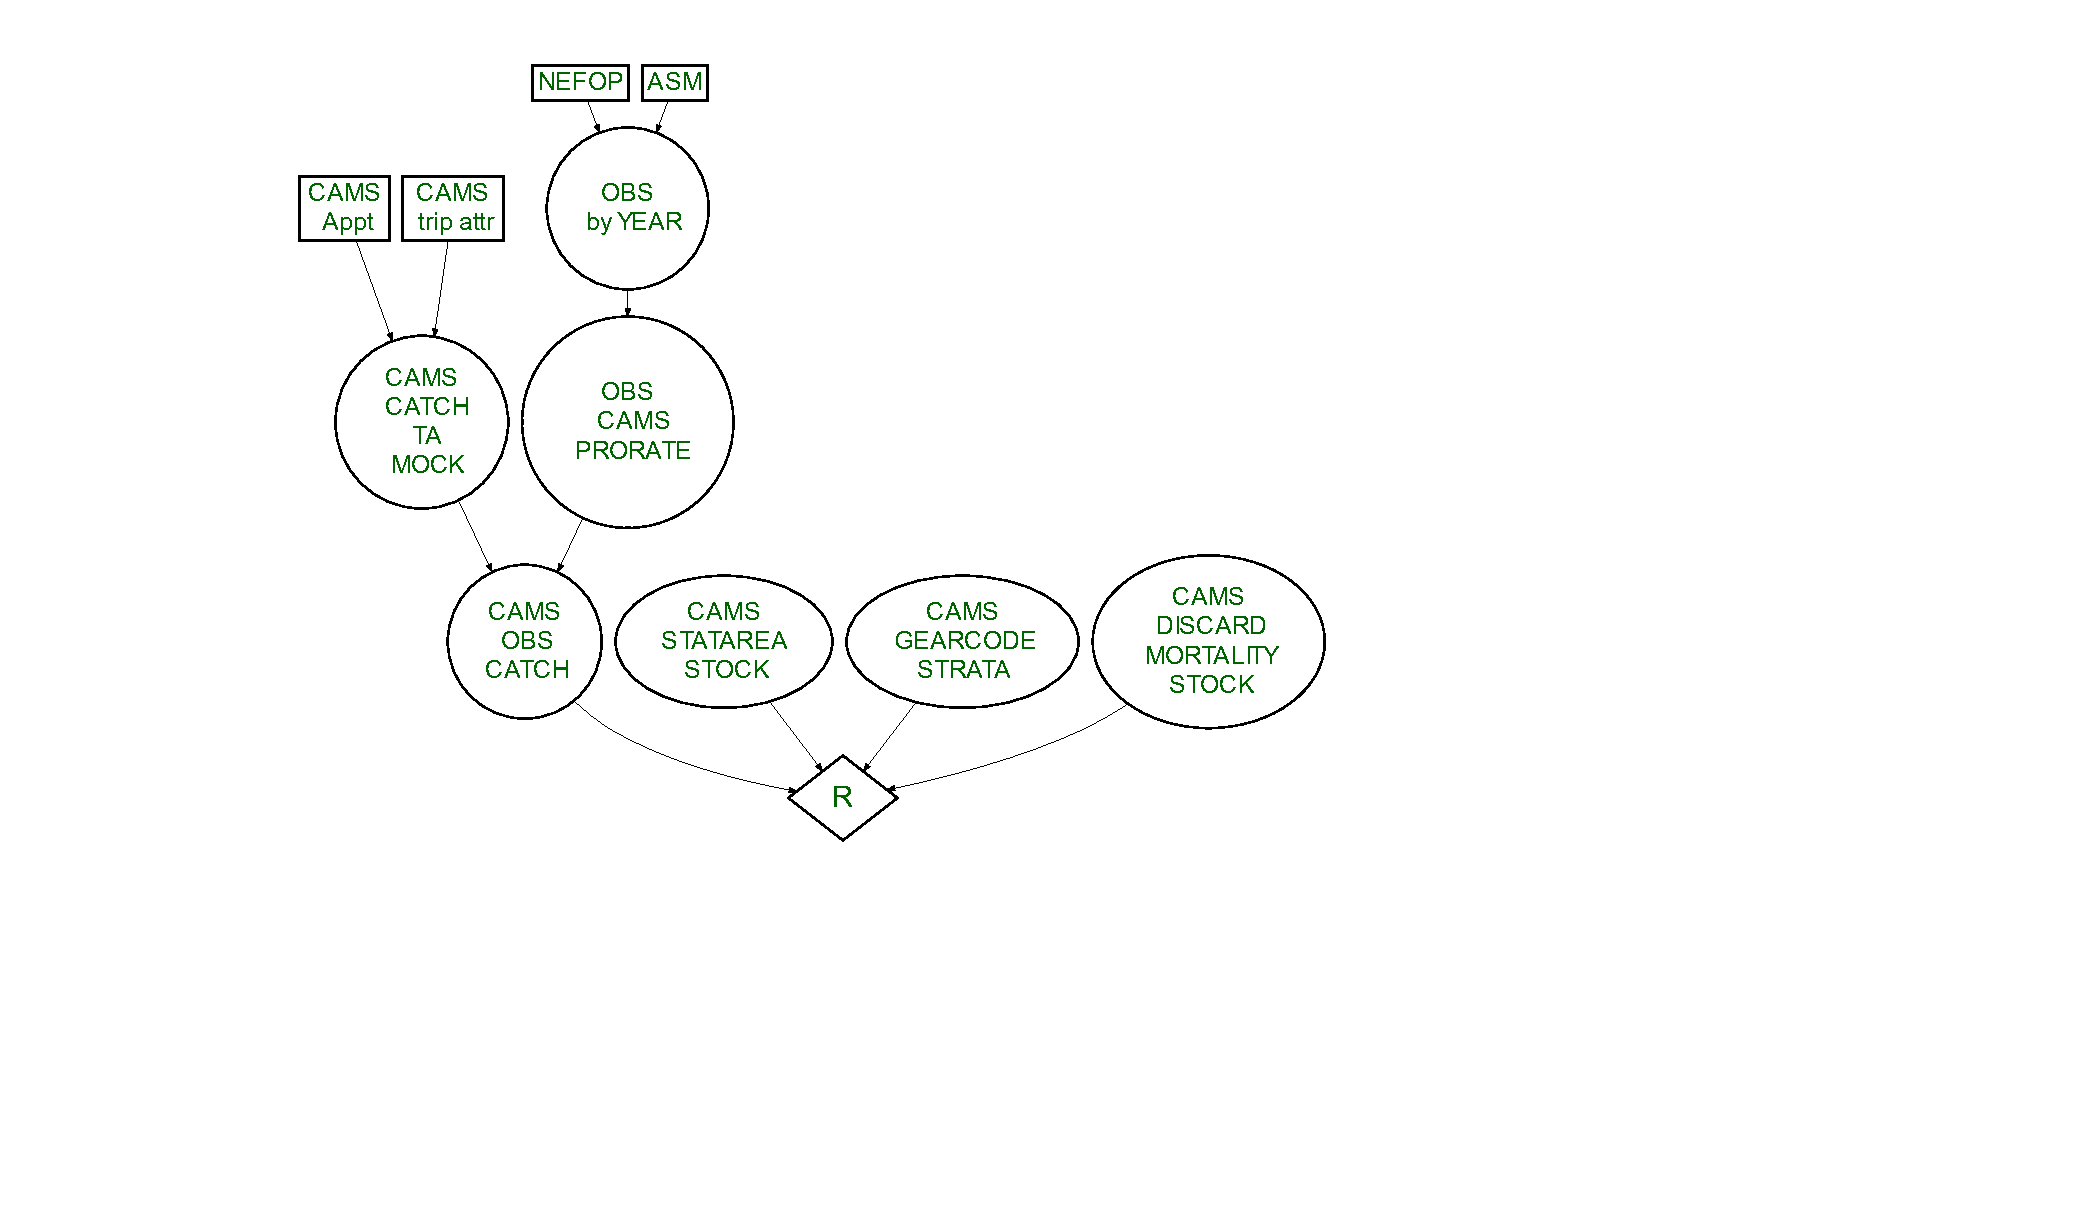
\includegraphics{discard_documention_beamer_files/figure-beamer/table_flow0-1.pdf}
\caption{Base tables (rectangle), Intermediary (circle), and Support
tables (Oval)}
\end{figure}

\end{frame}

\begin{frame}[fragile]{Tables created and steps to date}
\protect\hypertarget{tables-created-and-steps-to-date}{}

\textbf{Rates determine by observer reported values (gear, area, etc)}
Observed discards

\texttt{make\_obdbs\_table\_cams\_v2.sql}

created:

\begin{itemize}
\tightlist
\item
  \texttt{apsd.bg\_obdbs\_cams\_mock2018}
\item
  \texttt{apsd.bg\_obdbs\_cams\_mock2019}
\item
  \texttt{apsd.bg\_obdbs\_cams\_mock2020}
\end{itemize}

\end{frame}

\begin{frame}[fragile]{Prorated discards}
\protect\hypertarget{prorated-discards}{}

\textbf{Incomplete observed trips have missing `hauls' prorated by
observed information from that trip}

Prorate observed discards on unobserved hauls within a subtrip. This is
done by applying a ratio of kept all on the entire trip to kept all on
the unobserved hauls only

\[d_{total} = d_{observedhauls}*(1+KALL_{unobserved hauls}/KALL_{subtrip})\]

\texttt{make\_obdbs\_prorate.sql}

created:

\begin{itemize}
\tightlist
\item
  \texttt{apsd.obs\_cams\_prorate}

  \begin{itemize}
  \tightlist
  \item
    this table was made using \texttt{apsd.bg\_obdbs\_cams\_mock2018}
    and \texttt{apsd.bg\_obdbs\_cams\_mock2019}
  \end{itemize}
\end{itemize}

\end{frame}

\begin{frame}[fragile]{Use prorated observed discard values}
\protect\hypertarget{use-prorated-observed-discard-values}{}

\textbf{Trips with observer get reported/calculated observed discards of
that specific trip}

Match observed hauls to subtrips

\texttt{explore\_link3\_mesh\_match.sql}

This step matches on \texttt{AREA}, \texttt{GEAR} and \texttt{MESHGROUP}
(sm, lg, xlg). This is a hard match and will go awry if there is a
mismatch in the data.

\end{frame}

\begin{frame}[fragile]{Use prorated observed discard values (cont.)}
\protect\hypertarget{use-prorated-observed-discard-values-cont.}{}

tables created:

\begin{itemize}
\tightlist
\item
  \texttt{apsd.bg\_cams\_catch\_mock}

  \begin{itemize}
  \tightlist
  \item
    follows the steps layed out for mid-Atlantic discard estimation.
    \texttt{Gear}, \texttt{mesh}, \texttt{region},
    \texttt{half\ of\ year} CASE statements should be replaced at some
    point with table driven code.\\
  \item
    Utilizes the current apportionment table:
    \texttt{apsd.cams\_apport\_20201230}
  \end{itemize}
\item
  \texttt{apsd.bg\_obs\_cams\_tmp1}

  \begin{itemize}
  \tightlist
  \item
    links to \texttt{dmis.d\_match\_obs\_link} and
    \texttt{apsd.bg\_cams\_catch\_mock}; \textbf{multiple} subtrips
    only. 
  \end{itemize}
\item
  \texttt{apsd.bg\_obs\_cams\_tmp2} is used in the
  \texttt{squid\ example} and include all trips.
\end{itemize}

\end{frame}

\begin{frame}[fragile]{R functions}
\protect\hypertarget{r-functions}{}

\begin{itemize}
\tightlist
\item
  \texttt{get\_obs\_disc\_vals}
\item
  \texttt{make\_assumed\_rate}
\item
  \texttt{make\_bdat\_focal}
\item
  \texttt{run\_discard}
\end{itemize}

\end{frame}

\begin{frame}[fragile]{Running it}
\protect\hypertarget{running-it}{}

\begin{itemize}
\tightlist
\item
  refresh Oracle tables?
\item
  define species

  \begin{itemize}
  \tightlist
  \item
    generates SQL
  \end{itemize}
\item
  import to R

  \begin{itemize}
  \tightlist
  \item
    apply CAMS\_GEAR\_GROUP according to SPECIES
  \item
    apply STOCK STAT AREA according to SPECIES and stock (if needed)
  \end{itemize}
\item
  \texttt{run\_discard}

  \begin{itemize}
  \tightlist
  \item
    STRATA is assigned dynamically by species/stock using elements of
    the imported data
  \item
    If using \texttt{transition\ rates}, two time periods are defined
  \item
    Assumed (fallback rates) are defined as a subset of STRATA
  \end{itemize}
\item
  Apply Discard Mortality

  \begin{itemize}
  \tightlist
  \item
    Match by CAMS\_GEAR\_GROUP at the subtrip level
  \end{itemize}
\end{itemize}

\end{frame}

\begin{frame}{output}
\protect\hypertarget{output}{}

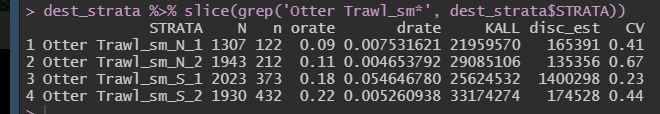
\includegraphics[width = \textwidth]{dest_strata_squid_ex.jpg}
\vspace{2cm} 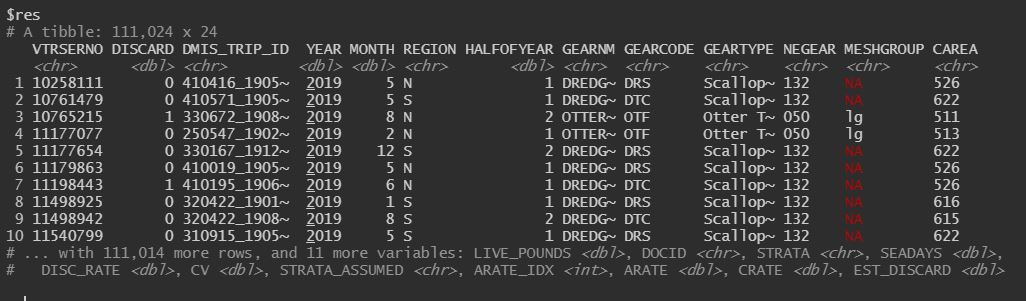
\includegraphics[width = \textwidth]{squid_ex_table.jpg}

\end{frame}

\begin{frame}{compare to ACL summary}
\protect\hypertarget{compare-to-acl-summary}{}

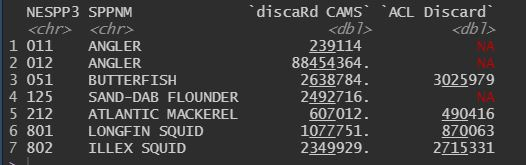
\includegraphics[width = \textwidth]{CAMS_discaRd_ACL_comparison.jpg}

\end{frame}

\begin{frame}[fragile]{TO DO}
\protect\hypertarget{to-do}{}

\begin{itemize}
\tightlist
\item
  utilize support tables

  \begin{itemize}
  \tightlist
  \item
    \texttt{CAMS\_GEAR\_GROUP} \textbf{DONE}
  \item
    \texttt{STAT\_AREAS} \textbf{DONE}
  \end{itemize}
\item
  add \texttt{SECTOR} for multispecies (see above) \textbf{DONE}
\item
  utilize discard mortality table (species/gear/mesh)
  \textbf{imminent..}
\item
  decide on time periods \textbf{Determined by STOCK/SPECIES}

  \begin{itemize}
  \tightlist
  \item
    Species with the same tiem period, e.g.~Calendar year, can be
    imported at once.
  \end{itemize}
\item
  decide on criteria for assumed (fallback) rates: how simplified must
  this be?
\item
  implement transitions (if using fixed time period) \textbf{DONE}
\item
  refine exact operational process
\end{itemize}

\end{frame}

\end{document}
